\section{Cross-compiling user-space libraries and applications}

\begin{frame}{Integrating user-space libraries and applications}
  \begin{itemize}
  \item One of the advantages of embedded Linux is the wide range of
    third-party libraries and applications that one can leverage in
    its product
  \item There's much more than U-Boot, Linux and Busybox that we can
    re-use from the open-source world
  \item Networking, graphics, multimedia, crypto, language
    interpreters, and more.
  \item Each of those additional software components needs to be
    cross-compiled and installed for our target
  \item Including all their dependencies
    \begin{itemize}
    \item Which can be quite complex as open-source encourages code
      re-use
    \end{itemize}
  \end{itemize}
\end{frame}

\begin{frame}{Concept of build system}
  \begin{itemize}
  \item Each open-source software project comes with its own set of
    scripts/files to control its configuration/compilation: its {\em
      build system}
    \begin{itemize}
    \item Detect if system requirements/dependencies are met
    \item Compile all source files, to generate
      applications/libraries, as well as documentation
    \item Installs build products
    \end{itemize}
  \item Most common build systems:
    \begin{itemize}
    \item Hand-written {\em Makefiles}
    \item {\em Autotools}: {\em autoconf}, {\em automake}, {\em libtool}\\
      \url{https://en.wikipedia.org/wiki/GNU_Autotools}
    \item {\em CMake}\\
      \url{https://cmake.org/}
    \item {\em Meson}\\
      \url{https://mesonbuild.com/}
    \item Language specific build systems for Python, Perl, Go, Rust,
      NodeJS, etc.
    \end{itemize}
  \end{itemize}
\end{frame}

\begin{frame}{Target and staging spaces}
  \begin{itemize}
  \item When manually cross-compiling software, we will distinguish
    two ``copies'' of the root filesystem
    \begin{enumerate}
    \item The target root filesystem, which ends up on our embedded
      hardware, which contains only what is needed for {\em runtime}
    \item The staging space, which has a similar layout, but contains
      a lot more files than the {\em target} root filesystem: headers,
      static libraries, documentation, binaries with debugging
      symbols. Contains what's needed for {\em building} code.
    \end{enumerate}
  \item Indeed, we want the root filesystem on the target to be as
    minimal as possible.
  \end{itemize}
  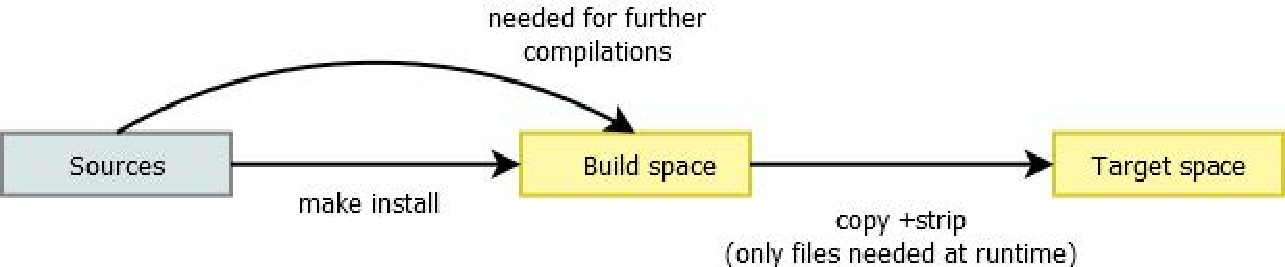
\includegraphics[width=\textwidth]{slides/sysdev-cross-compiling-user-space/source-build-target-spaces.pdf}
\end{frame}

\begin{frame}[fragile]{Cross-compiling with hand-written Makefiles}
  \begin{itemize}
  \item There is no general rule, as each project has a different
    set of Makefiles, that use a different set of variables
  \item Though it is common to use \code{make} standard variables:
    \code{CC} (C compiler path), \code{CXX} (C++ compiler path),
    \code{LD} (linker path), \code{CFLAGS} (C compiler flags),
    \code{CXXFLAGS} (C++ compiler flags), \code{LDFLAGS} (linker
    flags)
  \item \code{DESTDIR} for installation destination, sometimes
    \code{PREFIX} for execution location
  \item Common sequence
    \begin{block}{}
      {
        \begin{minted}{sh}
$ make CC=arm-linux-gcc CFLAGS=-I/path/to/headers \
       LDFLAGS=-L/path/to/libraries
$ make DESTDIR=/installation/path install
        \end{minted}
      }
    \end{block}
  \item Need to read the documentation (if any), read the Makefiles,
    and adapt to their behavior.
  \end{itemize}
\end{frame}

\begin{frame}[fragile]{Example: {\em uftp} native compilation}
  \begin{columns}
    \column{0.5\textwidth}
  \begin{block}{Download and extract}
    {\tiny
\begin{verbatim}
$ wget http://sourceforge.net/projects/uftp-multicast/files/\
       source-tar/uftp-5.0.tar.gz
$ tar xf uftp-5.0.tar.gz
$ cd uftp-5.0
\end{verbatim}
    }
  \end{block}

  \begin{block}{Build and install}
    {\tiny
\begin{verbatim}
$ make
cc  -g -Wall -Wextra [...]  -c server_announce.c
[...]
cc  -g -Wall -Wextra -o uftp uftp_common.o encrypt_openssl.o \
   server_announce.o [...] server_main.o \
   -lm -lcrypto  -lpthread
$ make DESTDIR=/tmp/test install
\end{verbatim}
    }
  \end{block}
    \column{0.5\textwidth}
  \begin{block}{Look at installed files}
    {\tiny
\begin{verbatim}
$ tree /tmp/test
/tmp/test/
└── usr
    ├── bin
    │   ├── uftp
    │   ├── uftpd
    │   ├── [...]
    └── share
        └── man
            └── man1
                ├── uftp.1
                ├── [...]

$ file /tmp/test/usr/bin/uftp
/tmp/test/usr/bin/uftp: ELF 64-bit LSB executable, x86-64
\end{verbatim}
    }
  \end{block}
\end{columns}
\end{frame}

\begin{frame}[fragile]{Example: {\em uftp} cross-compilation}
  \begin{block}{First attempt}
    {\scriptsize
\begin{verbatim}
$ export PATH=/xtools/gcc-arm-10.3-2021.07-x86_64-arm-none-linux-gnueabihf/bin:$PATH
$ make CC=arm-none-linux-gnueabihf-gcc
[...]
encryption.h:87:10: fatal error: openssl/rsa.h: No such file or directory
\end{verbatim}
    }
  \end{block}

  \begin{itemize}
  \item Build fails because {\em uftp} uses {\em OpenSSL}
  \item This is an optional dependency that can be disabled using the
    special \code{make} variable \code{NO_ENCRYPTION}
  \end{itemize}

  \begin{block}{Second attempt}
    {\scriptsize
\begin{verbatim}
$ make CC=arm-none-linux-gnueabihf-gcc NO_ENCRYPTION=1
arm-none-linux-gnueabihf-gcc  -g -Wall -Wextra [...]  -c server_announce.c
[...]
arm-none-linux-gnueabihf-gcc  -g -Wall -Wextra -o uftp uftp_common.o \
   encrypt_none.o server_announce.o [...] -lm   -lpthread
$ make DESTDIR=/tmp/target NO_ENCRYPTION=1 install
$ file /tmp/target/usr/bin/uftp
/tmp/target/usr/bin/uftp: ELF 32-bit LSB executable, ARM
\end{verbatim}
    }
  \end{block}
\end{frame}

\begin{frame}[fragile]{Example: {\em OpenSSL} cross-compilation}

  \begin{columns}
    \column{0.5\textwidth}
  OpenSSL has a hand-written \code{Configure} shell script that needs
  to be invoked before the build.

  \begin{block}{Download/extract}
    {\tiny
\begin{verbatim}
$ wget https://www.openssl.org/source/openssl-1.1.1q.tar.gz
$ tar xf openssl-1.1.1q.tar.gz
$ cd openssl-1.1.1q
\end{verbatim}
    }
  \end{block}

  \begin{block}{Configuration/build}
    {\tiny
\begin{verbatim}
$ CC=arm-none-linux-gnueabihf-gcc ./Configure --prefix=/usr \
    linux-generic32 no-asm
$ make
$ make DESTDIR=/tmp/staging install
\end{verbatim}
    }
  \end{block}
    \column{0.5\textwidth}
  \begin{block}{Installed files}
    {\tiny
\begin{verbatim}
$ tree /tmp/staging
└── usr
    ├── bin
    │   └── openssl
    ├── include
    │   ├── openssl
    │   │   ├── rsa.h
    │   │   └── [...]
    ├── lib
    │   ├── libcrypto.a
    │   ├── libcrypto.so -> libcrypto.so.1.1
    │   ├── libcrypto.so.1.1
    │   ├── [...]
    │   └── pkgconfig
    │       ├── libcrypto.pc
    │       └── [...]
    └── share
        ├── doc
        │   └── openssl
        └── man
\end{verbatim}
    }
  \end{block}
\end{columns}
\end{frame}

\begin{frame}[fragile]{Example: {\em uftp} with {\em OpenSSL} support}
  \begin{columns}
    \column{0.5\textwidth}
  \begin{block}{}
    {\tiny
\begin{verbatim}
$ make CC=arm-none-linux-gnueabihf-gcc
encryption.h:87:10: fatal error: openssl/rsa.h:
   No such file or directory
[...]
\end{verbatim}
    }
  \end{block}

  {\small It cannot find the header, let's add \code{CFLAGS} pointing
    to where OpenSSL headers are installed.}

  \begin{block}{}
    {\tiny
\begin{verbatim}
$ make CC=arm-none-linux-gnueabihf-gcc \
       CFLAGS=-I/tmp/staging/usr/include
[... build OK, but at link time ...]
ld: cannot find -lcrypto
\end{verbatim}
    }
  \end{block}

  {\small Compilation of object files work, but link fails as the
    linker cannot find the OpenSSL library. Let's add \code{LDFLAGS}
    pointing to where the OpenSSL libraries are installed.}

  \column{0.5\textwidth}

  \begin{block}{}
    {\tiny
\begin{verbatim}
$ make CC=arm-none-linux-gnueabihf-gcc \
       CFLAGS=-I/tmp/staging/usr/include \
       LDFLAGS=-L/tmp/staging/usr/lib
[... builds OK! ...]
$ make DESTDIR=/tmp/target install
\end{verbatim}
    }
  \end{block}

  {\small Now it builds and installs fine!}

  \begin{block}{}
    {\tiny
\begin{verbatim}
$ arm-none-linux-gnueabihf-readelf -d /tmp/target/usr/bin/uftp
[...]
 0x00000001 (NEEDED) Shared library: [libm.so.6]
 0x00000001 (NEEDED) Shared library: [libcrypto.so.1.1]
 0x00000001 (NEEDED) Shared library: [libpthread.so.0]
 0x00000001 (NEEDED) Shared library: [libc.so.6]
[...]
\end{verbatim}
    }
  \end{block}

  {\small We can indeed see that \code{uftp} is linked against the
    \code{libcrypto.so.1.1} shared library.}

\end{columns}
\end{frame}

\begin{frame}{Autotools}
  \begin{itemize}
  \item A family of tools, which associated together form a complete
    and extensible build system
    \begin{itemize}
    \item {\bf autoconf} is used to handle the configuration of the
      software package
    \item {\bf automake} is used to generate the Makefiles needed to
      build the software package
    \item {\bf libtool} is used to handle the generation of shared
      libraries in a system-independent way
    \end{itemize}
  \item Most of these tools are old and relatively complicated to use
  \item But they are used by a large number of software components,
    even though {\em Meson} is gaining significant traction as a
    replacement today
  \item See also
    \href{https://bootlin.com/doc/training/autotools/}{Bootlin
      Autotools training materials}
  \end{itemize}
\end{frame}

\begin{frame}{automake / autoconf / autoheader}
  \begin{center}
    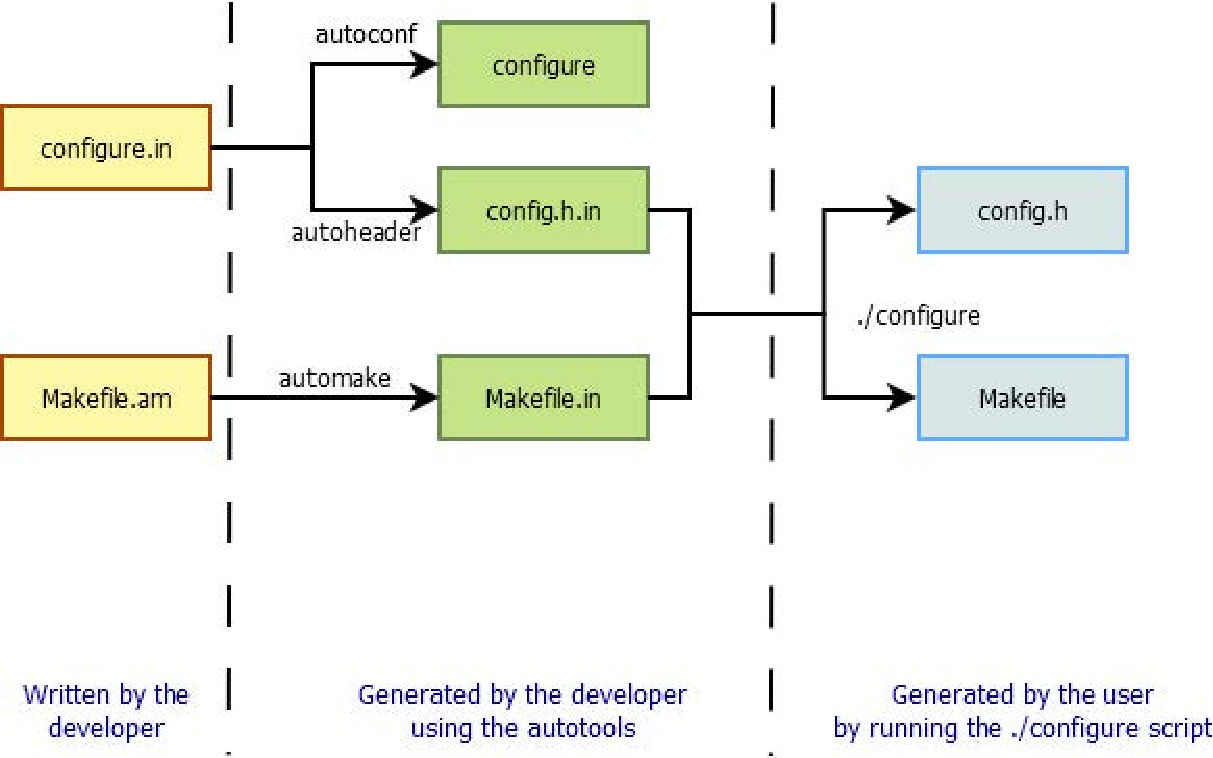
\includegraphics[height=0.8\textheight]{slides/sysdev-cross-compiling-user-space/autotools.pdf}
  \end{center}
\end{frame}

\begin{frame}{automake / autoconf}
  \begin{itemize}
  \item Files written by the developer
    \begin{itemize}
    \item \code{configure.in} describes the configuration options and
      the checks done at configure time
    \item \code{Makefile.am} describes how the software should be
      built
    \end{itemize}
  \item The \code{configure} script and the \code{Makefile.in} files
    are generated by \code{autoconf} and \code{automake} respectively.
    \begin{itemize}
    \item They should never be modified directly
    \item Software downloaded as a tarball: usually shipped
      pre-generated in the tarball
    \item Software downloaded from Git: no pre-generated files under
      version control, so they must be generated
    \end{itemize}
  \item The \code{Makefile} files are generated at configure time, before
    compiling
    \begin{itemize}
    \item They are never shipped in the software package.
    \end{itemize}
  \end{itemize}
\end{frame}

\begin{frame}{autotools usage: four steps}
  \begin{enumerate}
  \item Only if needed: generate \code{configure} and
    \code{Makefile.in}. Either using {\em autoreconf} tool, or
    sometimes an \code{autogen.sh} script is provided by the package
  \item {\bf Configuration:} \code{./configure}
    \begin{itemize}
    \item \code{./configure --help} is very useful
    \item \code{--prefix}: execution location
    \item \code{--host}: target machine when cross-compiling, if not
      provided, auto-detected. Also used as the cross-compiler prefix.
    \item Often \code{--enable-<foo>}, \code{--disable-<foo>},
      \code{--with-<foo>}, \code{--without-<foo>} for optional
      features.
    \item \code{CC}, \code{CXX}, \code{CFLAGS}, \code{CXXFLAGS},
      \code{LDFLAGS} and many more variables
    \end{itemize}
  \item {\bf Build:} \code{make}
  \item {\bf Installation:} \code{make install}
    \begin{itemize}
    \item \code{DESTDIR} variable for {\em diverted installation}
    \end{itemize}
  \end{enumerate}
\end{frame}

\begin{frame}[fragile]{Example: can-utils native compilation}
  \begin{columns}
    \column{0.5\textwidth}
  \begin{block}{Download}
    {\tiny
\begin{verbatim}
$ git clone https://github.com/linux-can/can-utils.git
$ cd can-utils/
$ git checkout v2021.08.0
$ ls -1 configure* *makefile*
configure.ac
GNUmakefile.am
\end{verbatim}
    }
  \end{block}

  {\small No \code{configure} and
    \code{GNUmakefile.in}, {\em autoreconf needed}.}

  \begin{block}{Autoreconf}
    {\tiny
\begin{verbatim}
$ autoreconf -i
$ ls -1 configure* *makefile*
configure
configure.ac
GNUmakefile.am
GNUmakefile.in
\end{verbatim}
    }
  \end{block}

  \column{0.5\textwidth}

  \begin{block}{Configuration}
    {\tiny
\begin{verbatim}
$ ./configure --prefix=/usr
$ ls -1 *makefile*
GNUmakefile
GNUmakefile.am
GNUmakefile.in
\end{verbatim}
    }
  \end{block}

  {\small We now have the \code{GNUmakefile}, we can build and install.}

  \begin{block}{Build/install}
    {\tiny
\begin{verbatim}
$ make
$ make DESTDIR=/tmp/test install
$ file /tmp/test/usr/bin/candump
/tmp/test/usr/bin/candump: ELF 64-bit LSB executable, x86-64
\end{verbatim}
    }
  \end{block}

\end{columns}
\end{frame}

\begin{frame}[fragile]{Example: {\em can-utils} cross-compilation}
  \begin{block}{}
    {\scriptsize
\begin{verbatim}
$ export PATH=/xtools/gcc-arm-10.3-2021.07-x86_64-arm-none-linux-gnueabihf/bin:$PATH
$ ./configure --prefix=/usr --host=arm-none-linux-gnueabihf
$ make
$ make DESTDIR=/tmp/target install
$ file /tmp/target/usr/bin/candump
/tmp/target/usr/bin/candump: ELF 32-bit LSB executable, ARM
\end{verbatim}
    }
    \end{block}

    Note: This is a simple example, as {\em can-utils} does not have
    any dependency other than the C library, and has a simple
    \code{configure.ac} file.
\end{frame}

\begin{frame}{CMake}
  \url{https://en.wikipedia.org/wiki/CMake}
  \begin{itemize}
  \item More modern build system, started in 1999, maintained by a
    company called {\em Kitware}
  \item Used by Qt 6, KDE, and many projects which didn't like {\em
      autotools}
  \item Perhaps losing traction these days in favor of {\em Meson}
  \item Needs \code{cmake} installed on your machine
  \item Based on:
    \begin{itemize}
    \item \code{CMakeLists.txt} files that describe what the
      dependencies are and what to build and install
    \item \code{cmake}, a tool that processes \code{CMakeLists.txt} to
      generate either Makefiles (default) or Ninja files (covered later)
    \end{itemize}
  \item Typical sequence, when using the {\em Makefile} backend:
    \begin{enumerate}
    \item \code{cmake .}
    \item \code{make}
    \item \code{make install}
    \end{enumerate}
  \end{itemize}
\end{frame}

\begin{frame}[fragile]{Example: {\em cJSON} native compilation}

  \begin{columns}
    \column{0.5\textwidth}
    \begin{block}{Download}
      {\tiny
\begin{verbatim}
$ git clone https://github.com/DaveGamble/cJSON.git
$ cd cJSON
$ git checkout v1.7.15
\end{verbatim}
      }
    \end{block}

    \begin{block}{Configure, build, install}
      {\tiny
\begin{verbatim}
$ cmake -DCMAKE_INSTALL_PREFIX=/usr .
$ make
$ make DESTDIR=/tmp/test install
\end{verbatim}
      }
    \end{block}
    \column{0.5\textwidth}
    \begin{block}{Installed files}
      {\tiny
\begin{verbatim}
$ tree /tmp/test
/tmp/test/
└── usr
    ├── include
    │   └── cjson
    │       └── cJSON.h
    └── lib64
        ├── cmake
        │   └── cJSON
        │       ├── cjson.cmake
        │       ├── cJSONConfig.cmake
        │       ├── cJSONConfigVersion.cmake
        │       └── cjson-noconfig.cmake
        ├── libcjson.so -> libcjson.so.1
        ├── libcjson.so.1 -> libcjson.so.1.7.15
        ├── libcjson.so.1.7.15
        └── pkgconfig
            └── libcjson.pc
\end{verbatim}
      }
    \end{block}
  \end{columns}
\end{frame}

\begin{frame}[fragile]
  \frametitle{Example: {\em cJSON} cross-compilation}
  % \frametitle was necessary here otherwise the \em string is invisible
  {\em cJSON} has no dependency on any other library, so
  cross-compiling it is very easy as only the C cross-compiler needs
  to be specified:
  \begin{block}{}
    {\scriptsize
\begin{verbatim}
$ cmake -DCMAKE_INSTALL_PREFIX=/usr -DCMAKE_C_COMPILER=arm-none-linux-gnueabihf-gcc .
$ make
$ make DESTDIR=/tmp/target install
$ file /tmp/target/usr/lib/libcjson.so.1.7.15
/tmp/target/usr/lib/libcjson.so.1.7.15: ELF 32-bit LSB shared object, ARM
\end{verbatim}
    }
  \end{block}
\end{frame}

\begin{frame}{CMake {\em toolchain file}}
  \begin{itemize}
  \item When cross-compiling with {\em CMake}, the number of arguments
    to pass to specify the paths to all cross-compiler tools,
    libraries, headers, and flags can become quite long.
  \item They can be grouped into a {\em toolchain file}, which defines
    {\em CMake} variables
  \item Can then be used with \code{cmake
      -DCMAKE_TOOLCHAIN_FILE=/path/to/toolchain-file.txt}
  \item Such a {\em toolchain file} is commonly provided by embedded
    Linux build systems: Buildroot, Yocto, etc.
  \item Facilitates cross-compilation using CMake
  \item \url{https://cmake.org/cmake/help/latest/manual/cmake-toolchains.7.html}
  \end{itemize}
\end{frame}

\begin{frame}{Meson}
  \url{https://en.wikipedia.org/wiki/Meson_(software)}
  \begin{itemize}
  \item The most modern one, written in Python
  \item Gaining big traction in lots of major open-source projects
  \item Processes \code{meson.build} + \code{meson_options.txt} and
    generates {\em Ninja} files
  \item {\em Ninja} is an alternative to \code{make}, with much
    shorter build times
  \item Needs \code{meson} and \code{ninja} installed on your machine
  \item Meson requires an {\em out-of-tree} build: the build directory
    must be distinct from the source directory
    \begin{enumerate}
    \item \code{mkdir build}
    \item \code{cd build}
    \item \code{meson ..}
    \item \code{ninja}
    \item \code{ninja install}
    \end{enumerate}
  \end{itemize}
\end{frame}

\begin{frame}[fragile]{Example: {\em ipcalc} native compilation}

  \begin{columns}
    \column{0.5\textwidth}
    \begin{block}{Download}
      {\tiny
\begin{verbatim}
$ git clone https://gitlab.com/ipcalc/ipcalc.git
$ cd ipcalc
$ git checkout 1.0.1
\end{verbatim}
      }
    \end{block}

    \begin{block}{Configuration, build, installation}
      {\tiny
\begin{verbatim}
$ mkdir build
$ cd build
$ meson --prefix /usr ..
$ ninja
$ DESTDIR=/tmp/test ninja install
\end{verbatim}
      }
    \end{block}

    \column{0.5\textwidth}

    \begin{block}{Installed files}
      {\tiny
\begin{verbatim}
$ tree /tmp/test
/tmp/test/
└── usr
    └── bin
        └── ipcalc
\end{verbatim}
      }
    \end{block}
  \end{columns}
\end{frame}

\begin{frame}[fragile]{Meson {\em cross file}}
  \begin{columns}
    \column{0.5\textwidth}
    \begin{itemize}
    \item In a similar manner to CMake's {\em toolchain file}, {\em
        Meson} has a concept of {\em cross file}
    \item Small text file that contains variable definitions telling
      {\em Meson} all details needed for cross-compilation
    \item Can be created manually, or may be provided by an embedded
      Linux build systems such as Buildroot or Yocto.
    \item \code{--cross-file} option of {\em Meson}
    \end{itemize}
    \column{0.5\textwidth}
    \begin{block}{Cross file example}
      {\tiny
\begin{verbatim}
[binaries]
c = 'arm-none-linux-gnueabihf-gcc'
strip = 'arm-none-linux-gnueabihf-strip'

[host_machine]
system = 'linux'
cpu_family = 'arm'
cpu = 'cortex-a9'
endian = 'little'
\end{verbatim}
      }
    \end{block}
  \end{columns}
\end{frame}

\begin{frame}[fragile]{Example: {\em ipcalc} cross-compilation}
    \begin{block}{}
      {\footnotesize
\begin{verbatim}
$ cat cross-file.txt
[binaries]
c = 'arm-none-linux-gnueabihf-gcc'
strip = 'arm-none-linux-gnueabihf-strip'

[host_machine]
system = 'linux'
cpu_family = 'arm'
cpu = 'cortex-a9'
endian = 'little'
$ mkdir build-cross
$ cd build-cross
$ meson --cross-file ../cross-file.txt --prefix /usr ..
$ ninja
$ DESTDIR=/tmp/target ninja install
$ file /tmp/target/usr/bin/ipcalc
/tmp/target/usr/bin/ipcalc: ELF 32-bit LSB executable, ARM
\end{verbatim}
      }
    \end{block}
\end{frame}

\begin{frame}{Distinction between {\em prefix} and {\em DESTDIR}}
  \begin{columns}
    \column{0.5\textwidth}
    \begin{itemize}
    \item There is often a confusion between {\em prefix} and {\em
        DESTDIR}
    \item Distinction is very important in cross-compilation context
    \item \code{prefix}: where the software will be executed from on the
      target
    \item \code{DESTDIR}: where the software is installed by the build
      system installation procedure. Allows to install in a different
      place than \code{prefix}, when creating a root filesystem for a
      different machine.
    \end{itemize}
    \column{0.5\textwidth}
    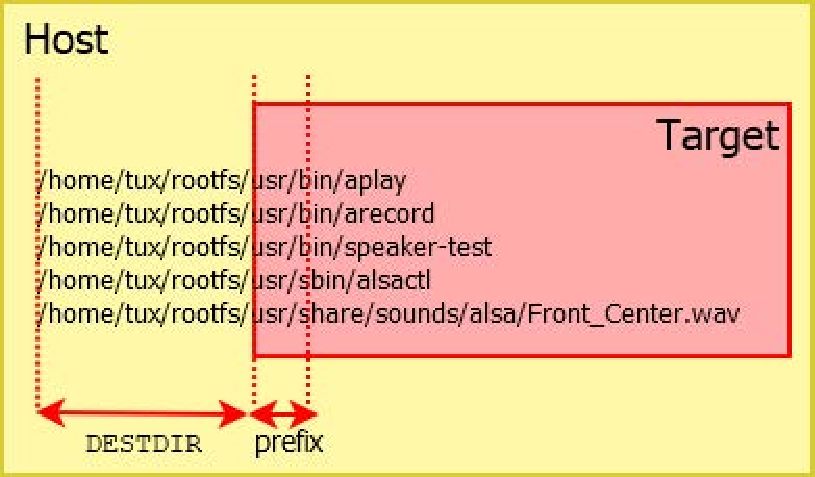
\includegraphics[width=\textwidth]{slides/sysdev-cross-compiling-user-space/destdir-and-prefix.pdf}
  \end{columns}
\end{frame}

\begin{frame}{pkg-config}
  \begin{itemize}
  \item \code{pkg-config} is a tool that allows to query a small
    database to get information on how to compile programs that depend
    on libraries
  \item \url{https://people.freedesktop.org/~dbn/pkg-config-guide.html}
  \item The database is made of \code{.pc} files, installed by default in
    \code{<prefix>/lib/pkgconfig/}.
  \item \code{pkg-config} is often used by {\em autotools}, {\em
      CMake}, {\em Meson} to find libraries
  \item By default, \code{pkg-config} looks in
    \code{/usr/lib/pkgconfig} for the \code{*.pc} files, and assumes
    that the paths in these files are correct.
  \item \code{PKG_CONFIG_LIBDIR} allows to set another location for the
    \code{*.pc} files.
  \item \code{PKG_CONFIG_SYSROOT_DIR} allows to prepend a directory to the
    paths mentioned in the \code{.pc} files and appearing in the
    \code{pkg-config} output.
  \end{itemize}
\end{frame}

\begin{frame}[fragile]{pkg-config example for native compilation}
  \begin{block}{}
    {\scriptsize
\begin{verbatim}
$ pkg-config --list-all
openssl                        OpenSSL - Secure Sockets Layer and cryptography libraries and tools
zlib                           zlib - zlib compression library
blkid                          blkid - Block device id library
cairo-script                   cairo-script - script surface backend for cairo graphics library
cairo-pdf                      cairo-pdf - PDF surface backend for cairo graphics library
xcb-xinput                     XCB XInput - XCB XInput Extension (EXPERIMENTAL)
libcurl                        libcurl - Library to transfer files with ftp, http, etc.
[...]
$ pkg-config --cflags --libs openssl
-lssl -lcrypto
$ pkg-config --cflags --libs cairo-script
-I/usr/include/cairo -I/usr/include/libpng16 -I/usr/include/freetype2 -I/usr/include/harfbuzz
[...] -lcairo -lz
\end{verbatim}
    }
  \end{block}
\end{frame}

\begin{frame}[fragile]{pkg-config example for cross-compilation}
  \begin{block}{Use \code{PKG_CONFIG_LIBDIR}}
    {\scriptsize
\begin{verbatim}
$ export PKG_CONFIG_LIBDIR=/tmp/staging/usr/lib/pkgconfig
$ pkg-config --list-all
openssl                        OpenSSL - Secure Sockets Layer and cryptography libraries and tools
libssl                         OpenSSL-libssl - Secure Sockets Layer and cryptography libraries
libcrypto                      OpenSSL-libcrypto - OpenSSL cryptography library
$ pkg-config --cflags --libs openssl
-I/usr/include -L/usr/lib -lssl -lcrypto
\end{verbatim}
    }
  \end{block}

  The \code{-L/usr/lib} is incorrect, we need to use
  \code{PKG_CONFIG_SYSROOT_DIR}.

  \begin{block}{Use \code{PKG_CONFIG_SYSROOT_DIR}}
    {\scriptsize
\begin{verbatim}
$ export PKG_CONFIG_SYSROOT_DIR=/tmp/staging/
$ pkg-config --cflags --libs openssl
-I/tmp/staging/usr/include -L/tmp/staging/usr/lib -lssl -lcrypto
\end{verbatim}
    }
  \end{block}
\end{frame}

\setuplabframe
{Cross-compiling applications and libraries}
{
  Time to start the practical lab!
  \begin{itemize}
  \item Manual cross-compilation of several open-source libraries and
    applications for an embedded platform.
  \item Learning about common pitfalls and issues, and their
    solutions.
  \item This includes compiling {\em alsa-utils} package,
    and using its \code{speaker-test} program to test that
    audio works on the target.
  \end{itemize}
}
